\section{Metodología}
    El primer paso a realizar en esta investigación es recrear el código de John A. Bullinaria,
    para esto se va a utilizar el repositorio de Optical Digits, al momento de obtener estos datos
    ya se va a poder comenzar con la programación en Python.

    Al momento de comprobar que el código funciona como el algoritmo de John, se realizarán modificaciones
    que permitirán repartir las tazas de aprendizaje con estos valores.

    Para obtenerlo se usarán metodologías como el Backpropagation y funciones de activación tal como la Sigmoidal.

    Cuando los dos proyectos se tengan, se realizar\'a una comparación, donde se vera cual de estos dos experimentos
    es más eficaz en proyectos de la vida real.
    
\section{Cronograma de Actividades}

    \begin{figure}[H]
        \centering
        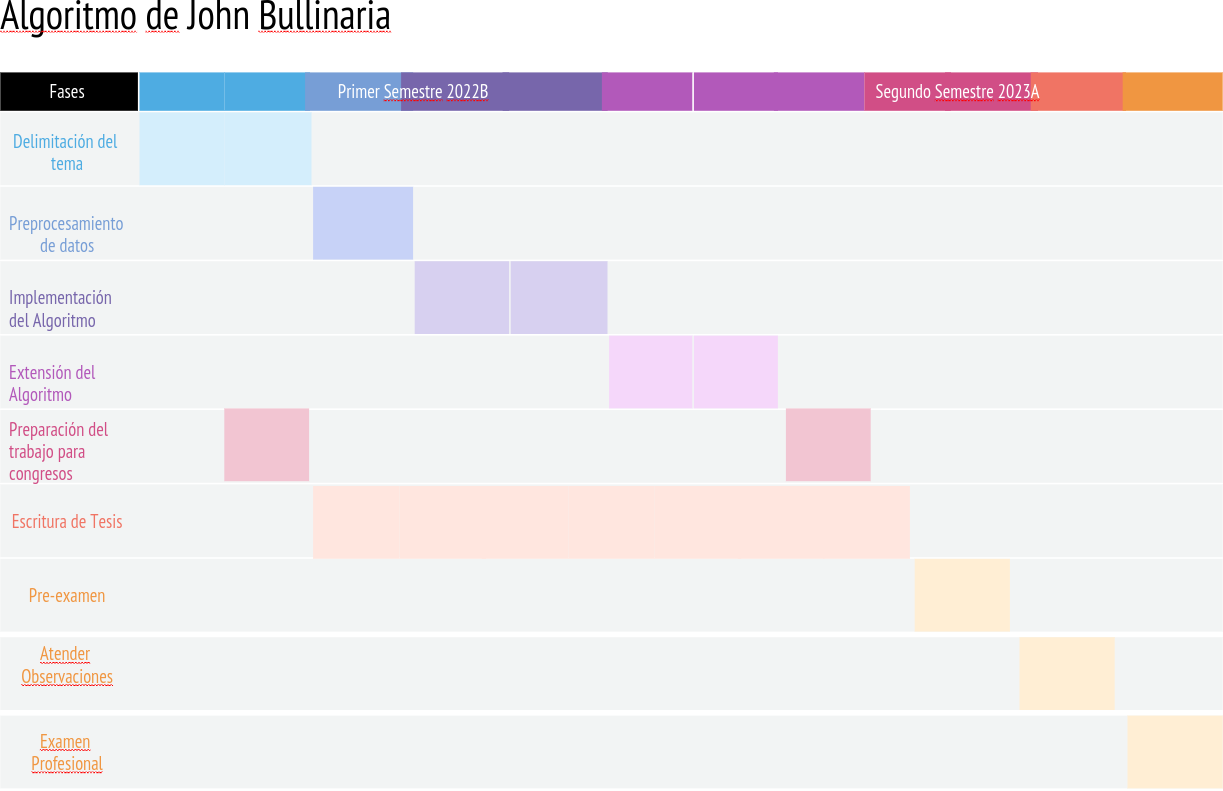
\includegraphics[width=\columnwidth]{diagramaGantt.png}
        \caption{Diagrama de Gantt}
        \label{fig:fig3}
    \end{figure}

\section{Organización del Capitulado}
	En el capitulo 2 se ver\'a lo que es el aprendizaje humano y el aprendizaje incremental con sus algoritmos, se describirán las redes neuronales artificiales.

En el capitulo 3 se implementar\'a el articulo de John A. Bullinaria, como funciona, resultado que da al pasar los datos que dice para comprobar que funciona como menciona en su art\'iculo. En el capitulo 4 se explicar\'a como se hará la modificación a su algoritmo, cuantas capas se van a poner, como se van a repartir las tazas de aprendizaje.

Posteriormente en el capitulo 5 se mostrar\'a una comparación de los resultados de ambos trabajos. En el capitulo 6 se verán las conclusiones y trabajo futuro.
